\documentclass[
    DIV12,
    cleardouble=plain,
    headings=normal,
    pdftex,
    headexclude,footexclude,
    final
]{scrreprt}

\usepackage{spreadtab}
\usepackage{xspace}
\usepackage{ngerman}
\usepackage[latin1]{inputenc}
%\usepackage[T1]{fontenc}
\usepackage[pdftex]{graphicx}
\usepackage[bookmarks]{hyperref}
\usepackage{scrpage2}
\usepackage{longtable}
\usepackage{caption}
\usepackage{pgfplots}
\usepackage{float}
\usepackage{xcolor}
\usepackage{colortbl}
\usepackage{relsize}
\usepackage{fancyvrb}

\graphicspath{{./}{./Pics/}}

% #################################################################

\hyphenation{Cha-otn-gsch-werl}
\setlength\headheight{1.75cm}

\ihead{\small{Hochschule Hof}}
\chead{}
\ohead{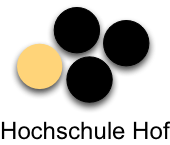
\includegraphics[height=0.05\textheight]{LogoGelb.png}}
\pagestyle{scrheadings}


\setcounter{secnumdepth}{5}
\setcounter{tocdepth}{5}
\renewcommand{\arraystretch}{1}

\parskip0.5\baselineskip plus 0.125\baselineskip minus 0.25\baselineskip
\parindent0em

% #################################################################

\def\SECH{S\kern-.075em \lower.5ex\hbox{E}\kern-0.05em CH\xspace}
\def\SEACH{S\kern-.075em \lower.5ex\hbox{E}\kern-0.05em ACH\xspace}

% #################################################################

%\automark[section]{chapter}

\titlehead{\begin{center}
\includegraphics[width=5cm]{fh_logo}\end{center}}
\title{
  \SECH--Tag--EEXCESS--Browser \\[1em]
  Programming Guide\\
Spezifikation, Konstruktion
}

\author{Prof. Dr. Peter St�hr \and Gottfried von Recum \and Alexander P�hlmann \and Tim Pohrer \and Lothar M�dl \and Burak Erol \and Brian Mairh�rmann \and Andreas Netsch \and Philipp Winterholler \and Patrick B�ttner \and Andreas Ziemer}
\date{Version 0.1.1}

% #################################################################


\begin{document}
\maketitle
\pagenumbering{roman}
\tableofcontents

\listoftables

\newpage
\pagenumbering{arabic}

\part*{Einleitung}
\chapter*{�ber dieses Dokument}

Dieses Dokument dient als Container f�r die im Lauf der
Arbeiten an dem \SECH--Projekt entstehenden Unterlagen. Die
Quellen f�r dieses Dokument liegen auf GutHub unter der URL
\url{https://github.com/SECH-App}.

Das Dokument muss von den bearbeitenden Gruppen parallel zu den
Entwicklungsarbeiten weiterentwickelt werden. 

Aktuell beschreibt das Dokument den Entwicklungsstand zum
Wintersemester 2015 und besteht aus folgenden Teilen:
\begin{enumerate}
     \item Einf�hrung in die Programmierung eines EEXCESS Clients.
     \item Spezifikation der beiden Teilsysteme.
     \item Konstruktion der beiden Teilsysteme.
\end{enumerate}


\chapter{\SECH--Browser}

\section{Projektziel}
Das Web besteht aus einer Vielzahl von Seiten mit
Informationen. Betrachtet man diese Seiten genauer, so stellt man
fest, dass ihr informationstragender Inhalt praktisch immer statisch
ist.  Er wird Zeitpunkt der Erstellung der Web--Seite von einem Autor
festgelegt und bleibt bis zum n�chsten Update in genau dieses
Zustand. Auch wenn die Seiten dynamisch generiert werden, der daf�r
verwendete Inhalt ist vorher von einem Autor geliefert worden.  Dass
diese Informationen statisch sind bedeutet auch, dass die Seiten f�r
alle Betrachter weltweit identisch sind.

Ziel des \SECH--Browsers ist es, diese statische Pr�sentation der
Informationen aufzuheben und die von einem Autor vorgegebenen Inhalte
automatisch um benutzerspezifische Informationen, den
\emph{\SECH--Annotations}\footnote{\SECH steht dabei f�r \textbf{S}elf
  \textbf{E}mbeding \textbf{C}haracteristic \textbf{H}yperlinks.}, zu
erg�nzen. Er folgt damit der Idee des \glqq taking the content to the
user\grqq\footnote{http://eexcess.eu} des EEXCESS--Projektes.


Die Auswahl der zus�tzlichen Informationen wird dabei von dem
\SECH--Browser, also dem Client, und nicht dem Server
vorgenommen. Personenbezogene Daten verlassen also nur dann den
eigenen Rechner, wenn es f�r die Suche nach den Daten der
\SECH--Annotations zwingend notwendig ist. Somit ist ein Maximum an
Datenschutz gegeben.

In der ersten Version basiert die Erzeugung der \SECH--Annotations
durch den \SECH--Brwoser auf Informationen, die der Seitenautor in
einem speziellen Format im Text hinterlegt hat. Diese Informationen,
die \SECH--Tags, verwendet der \SECH--Browser dazu, benutzerspezifische
Anfragen an eine Wissensquelle, beispielsweise dem Privacy--Proxy des
EEXCESS--Projektes (\url{http://eexcess.eu}), zu stellen und mit den
Ergebnissen die urspr�ngliche Darstellung der WWW--Seite zu
erg�nzen. 

In den weiteren Entwicklungsschritten soll der \SECH--Browser dann die
f�r die Erzeugung der \SECH--Annotations notwendigen Informationen
selbst�ndig aus den Textinhalten ableiten. Daf�r k�nnen dann
beispielsweise Techniken aus den Bereichen des Text-- beziehungsweise
Opinion--Minings verwendet werden.

\subsection{Anwendungsszenarien}
Im folgenden soll an Hand von einigen Beispielen dargestellt werden,
wie die zus�tzlichen Funktionalit�ten des \SECH--Browsers den Anwender
unterst�tzen k�nnen.

\subsubsection{Fremdenverkehr}
Web--Seiten von Fremdenverkehrsverb�nden werden von einer 
Vielzahl von verschiedenen Benutzergruppen besucht:
\begin{itemize}
     \item Besucher, die im n�heren Umkreis leben.
     \item Besucher von weiter her.
     \item Besuchern mit unterschiedlichen Muttersprachen.
     \item Besucher verschiedener Altergruppen.
     \item ...
\end{itemize}
Die verschiedenen Benutzergruppen haben in der Regel auch verschiedene
Anforderungen an die zur Verf�gung gestellten Informationen:
\begin{itemize}
     \item Ein Besucher, der nicht im n�heren Umkreis lebt, ben�tigt
    in der Regel eher Informationen �ber die Hotels des Gebietes als ein
    Besucher aus dem Umkreis.
     \item W�hrend Jugendliche sich eher f�r die Angebote aus dem Bereich
    der Fun--Sport--Arten interessieren, k�nnten Senioren eher an
    Informationen �ber die kulturellen Angebote der Region
    interessiert sein.
     \item Fremdsprachige Benutzer sollten vorrangig Informationen in
    ihrer Landessprache pr�sentiert werden.
\end{itemize}

Liegt ein gutes Design der Web--Seite vor, k�nnen die Besucher weitere Teile
der f�r sie relevanten Daten durch entsprechende Verlinkungen auf
andere Web--Seiten finden. Aber auch diese zus�tzlichen Informationen
sind statisch, f�r alle Besucher der Seite identisch und somit nicht
an die Bed�rfnisse der einzelnen Besucher angepasst.

Wie man sieht ist es auch in diesem Anwendungsfall f�r den Besucher
der Seite hilfreich, wenn der \SECH--Browser an Hand der ihm bekannten
benutzerspezifischen Informationen selbst�ndig erkennt, welche
zus�tzlichen Informationen f�r den Besucher interessant sein k�nnten
und diese dann entsprechend aufbereitet darstellen.

\subsubsection{Noch einer}

\section{Aufgabenstellung Wintersemester 2015/16}
Die im Wintersemester 2015/16 zu entwickelnde Version des
\SECH--Browsers umfasst folgende Schritte:
\begin{enumerate}
     \item Erstellung eines iOS--Programms zur Darstellung von
    Web--Seiten.
     \item Erstellung eines iOS/OS X Programms zur Generierung von
    Anfragen an den Privacy--Proxy des EEXCESS--Projekts und der
    Darstellung der jeweiligen Antworten.
     \item Definition der Syntax und Semantik des \SECH--Tags
    zur Beschreibung der vom Autor vorgegebenen Informationen zur
    Erstellung einer \SECH--Annotation.
     \item Erzeugung der um benutzerorientierte Informationen
    angereicherten Anfragen f�r den Privacy--Proxy.
     \item Integration der einzelnen Teilsysteme in einen lauff�higen
    Prototypen. 
\end{enumerate}
F�r die Software--Bausteine sind entsprechende Spezifikations--,
Konstruktions-- und Testdokumente zu erstellen. Diese Dokumente
orientieren sich an den Inhalten der Vorlesung \glqq Software
Engineering II\grqq.
 
Erweiterungen, wie beispielsweise
\begin{enumerate}
     \item Rating des Benutzers �ber die G�te der \SECH--Annotations einholen;
     \item Verwendung des Ratings um darauf folgende, �hnliche
    \SECH--Annotations zu verbessern;
\end{enumerate}
k�nnen in das Projekt einflie�en.
\chapter{Einführung in die Programmierung eines EEXCESS--Clients}
\section{Grundlegendes}
Die Kommunikation eines Clients mit dem EEXCESS--Server basiert auf
dem Austausch von JSON--Objekten. Im Rahmen des
\SECH--Browser--Projektes werden nur die Dienste des
Privacy--Proxy--Service\footnote{Im Folgenden mit PP--Service
  abgekürzt.}  in Anspruch genommen. Die dafür benötigten
JSON--Objekte sind in der Online--Dokumentation des EEXCESS--Projektes
auf GitHub beschrieben.

\section{Informationsanfrage}
Informationsanfragen an den PP--Server geschehen in der Regel in zwei
Schritten.

\begin{figure}[ht]
    \centering
    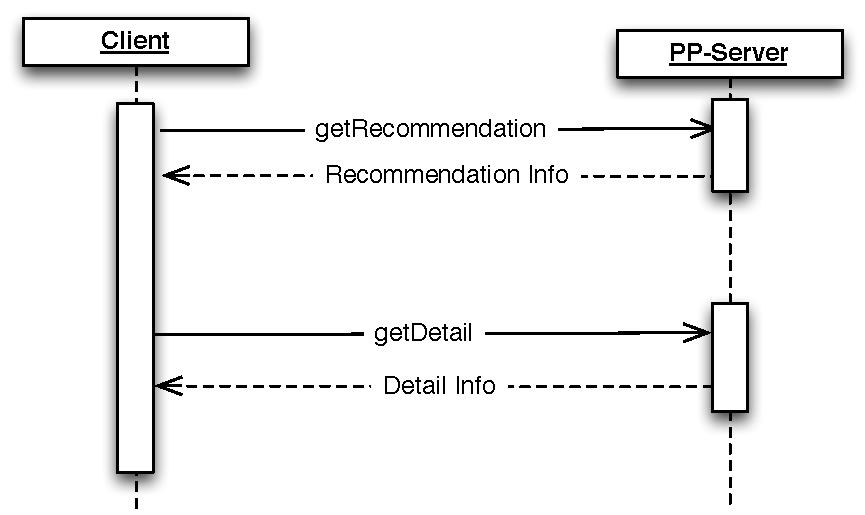
\includegraphics[width=0.75\textwidth]{clientServerComm}
    \caption{Beispiel für Informationsanfrage an den EEXCESS PP--Service}
    \label{fig:clientServerEEXCESS}
\end{figure}

Im ersten Schritt wird eine durch Suchparameter beschriebene
\Verb|/recommend|--Anfrage an der Server gestellt. Die Antwort darauf
besteht aus einem JSON--Objekt. Es enthält, neben den eigentlichen
Ergebnissen der Suchanfrage, auch eine eineindeutige ID zur späteren
Referenzierung der Anfrage. Die zurückgelieferten Ergebnisse bestehen
ihrerseits wieder aus verschiedenen Elementen, unter anderem einem
Titel der das Element näher beschreibt, einer URI die angibt wo das
Objekt gespeichert ist und einer eineindeutigen ID zur Referenzierung
des Objekts. Diese Informationen würden bereits ausreichen, um die einzelnen
Ergebnisse der Suchanfrage aus dem Netz zu laden. Da der Benutzer aber
selber entscheiden soll, ob die angezeigten Zusatzinformationen für
ihn interessant sein könnten, muss er vor der Darstellung eine Auswahl
treffen können. Dies ist anhand des Titels in der Regel nur schwer
möglich!

In einem zweiten, optionalen Schritt kann daher für jedes Ergebnis
einer \Verb|/recommend|--Anfrage eine detaillierte Kurzbeschreibung
vom PP--Server abgerufen werden. Der dafür vorgesehene
\Verb|/getDetails|--Befehl übergibt die ID der Suchanfrage und die
\Verb|documentBadge|--Informationen des ursprünglichen Ergebnisses an
den PP--Server und bekommt, falls bei der Datenquelle hinterlegt, eine
Kurzbeschreibung des Ergebnisses. An Hand dieser Kurzbeschreibung kann
der Anwender dann entscheiden, ob das eigentliche Informations--Objekt
über die zugeordnete URI geladen werden soll oder nicht.

\subsection{\texttt{/recommend}--Anfrage im \SECH--Browser Projekt}
Ein minimales JSON--Objekt für eine \Verb|/recommend|
Anfrage an den PP--Server besteht aus 3~Teilen:
\begin{enumerate}
     \item Den \Verb|origin| Informationen, die den Client näher beschreiben.
     \item Dem \Verb|loggingLevel|, der angibt ob der PP--Server die
    Anfragen aufzeichnen darf oder nicht.
    \item Den \Verb|contextKeywords|, die die eigentlichen
   Suchbegriffe beinhalten.
\end{enumerate}

Über weitere Parameter können die \Verb|/recommend|--Anfrage noch
genauer definiert werden. Im \SECH--Browser werden folgende
Parameter verwendet:
\begin{enumerate}
     \item \Verb|numResults|, um die Anzahl der vom PP-Server
    zurückgegebenen Resultate begrenzen zu können.
     \item Das \Verb|isMainTopic| Attribut der \Verb|contextKeywords|
    Einträge, um bei mehreren Suchparametern eine Priorisierung
    durchführen zu können.
     \item \Verb|interests|, um die Anfragen genauer an die Vorlieben
    des Benutzers anpassen zu können.
     \item \Verb|languages|, um bevorzugt \SECH--Annotations in der
    Muttersprache des Benutzers zu verwenden.
     \item \Verb|timeRange|, um die \SECH--Annotations zeitlich
    eingrenzen zu können.
\end{enumerate}

%Falls vom PP--Server unterstützt, sollen auch folgende Parameter zur
%näheren Beschreibung der Suchanfrage verwendet werden:
%\begin{itemize}
%     \item \Verb|ageRange|
%     \item \Verb|gender|
%     \item \Verb|address|
%\end{itemize}
\part*{Spezifikation}
\chapter*{EEXCESS-Browser}

\section{Funktionalit�ten}

\begin{itemize}
	\item WebView
	\item Back/Forward Button
	\item Lesezeichen
	\item Home-Button
	\item AdressBar
	\item Reload
	\item Men�
\end{itemize}

Mit Hilfe der WebView ist es m�glich, die gew�nschte Webseite anzuzeigen. Befindet man sich auf einer Webseite mit SECH-Tags, so erh�lt man zu diesen zus�tzliche Informationen.

Durch den Back bzw. Forward- Button springt man eine Seite zur�ck bzw. vor. 

In der AdressBar gibt man die URL der gew�nschten Webseite an. Nach einem Klick in die WebView wird die URL gepr�ft und die Seite geladen.

Bei Eingabe eines Suchbegriffs z.B. "Bamberg" wird man auf www.google.de weitergeleitet.

Nach einem Klick auf das Lesezeichensymbol wird die aktuelle Webseite durch Eingabe eines gew�hlten Namens zu den Favoriten hinzugef�gt. 

Durch Klick auf den Home-Button wird man auf die aktuell festgelegte Startseite weitergeleitet.

Durch den Reload-Button ist es m�glich, die aktuelle Webseite neu zu laden.
\part*{Konstruktion}
\chapter{Erstellung des Sechobjects}

\begin{figure}
	\centering
	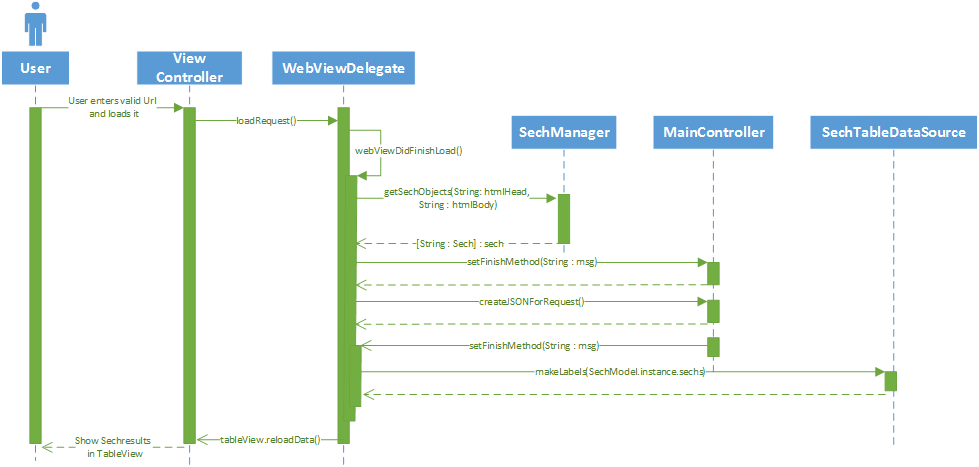
\includegraphics[scale=0.6]{sechobject.png}
	\caption{Ablauf der Erstellung eines \SECH-Objektes}
	\label{fig:SECH-Objekt Erstellung}
\end{figure}

Sobald der User eine gültige URL eingibt und lädt, wird die Laderoutine \Verb|loadRequest()|
angestoßen. Ist die Seite fertig geladen wird in der Delegatemethode \Verb|webViewDidFinishLoad()|
des WebViewDelegates das Auslesen bzw. Laden der \SEARCH-Tags begonnen.

Dem \SEARCH-Manager wird der HTML-Head und Body der eben geladenen Website übergeben und es
werden mit Hilfe des HTMLManagers \SEARCH-Objekte erstellt. Diese \SEARCH-Objekte werden in einem
Dictionary zurückgegeben.

Sobald ein \SECH-Object-Dictionary zurückgegeben wurde, werden die Ergebnisse gerankt und an den SechTableDataSource übergeben. Anschließend wird mit reloadData() die Tabelle der \SECH-Tags im ViewController befüllt.

\end{document}
